\chapter{Applied Methods}\label{chapter:applied-methods}

This chapter documents how the prototypical micro-frontend architecture was built step by step—the first section centers around identifying bounded contexts and deriving the micro-frontends from them. The following section is about the prototypical implementation of the micro-frontend architecture. After implementing the architecture, the communication patterns between the micro-frontends were analyzed and implemented. The next section centers around developing a shared caching layer. The last section focuses on a mechanism to remove fields from a GraphQL query by utilizing the Apollo Client's in-memory cache. This chapter ends by showing how query reduction works in practice.

\section{Identification of micro-frontends}\label{section:applied-methods:identification-micro-frontends}

The first step before starting to implement the micro-frontend architecture was to identify the parts of the legacy application that should be extracted into microservices and micro-frontends. The application is a large software monolith with a single database. In collaboration with the product owner, the bounded contexts of the legacy application were identified as candidates for micro-frontends and microservices. 

\bigskip

\noindent The complete legacy application can't be prototyped in the course of this master thesis, therefore the three most important bounded contexts were identified. The first bounded contexts to implement are the following:

\begin{itemize}
  \item User
  \item Sales
  \item Contact
  \item Dashboard
\end{itemize}
\section{Implementing a prototypical micro-frontend architecture}\label{section:applied-methods:prototypical-implementation}

The first step was to implement a prototypical micro-frontend application to evaluate the hypothesis. The base architecture was developed to lay the groundwork for later use in a production environment. The micro-frontends are integrated using client-side integration, more precisely, run-time integration. The integration strategy was implemented with Webpack's Module Federation, which was described in more detail in Section \ref{subsection:background:micro-frontend:module-federation}. The majority of the implementation is written in Angular. One micro-frontend was implemented in React to showcase the technology agnosticism of the caching strategy. The prototype contains an application shell that consumes the other micro-frontends. The architecture is divided into nine widgets that display only simple data and four complex single-page applications. The four \acp{SPA} are Dashboard, Contact, Sales, and User.

\bigskip

\noindent The library Nx from the company Nwrl is used for managing the micro-frontends and libraries in a single monorepo. An essential feature of Nx is the support for monorepos, which is the perfect match for managing micro-frontend applications. It offers support and tooling for almost any \ac{JS} framework and can be customized with plugins. Multiple related projects can be managed in a single workspace. Additionally, it ensures that every project uses the same version of a dependency across the workspace. Besides, Nx offers helper functions for working with Module Federation in micro-frontends. \cite{misc:-:applied-methods:intro-to-nx}

\bigskip

\noindent A rough overview of the architecture is shown in Figure \ref{fig:applied-methods:prototype-micro-frontend-architecture}. It shows a wireframe of the structure of the application. The icons inside the squares represent the \ac{JS} framework used. Each widget is a separate micro-frontend that exposes a remote module through Module Federation, which is then consumed by the Dashboard micro-frontend.

\ifshowImages
\begin{figure}[H]
  \centering
  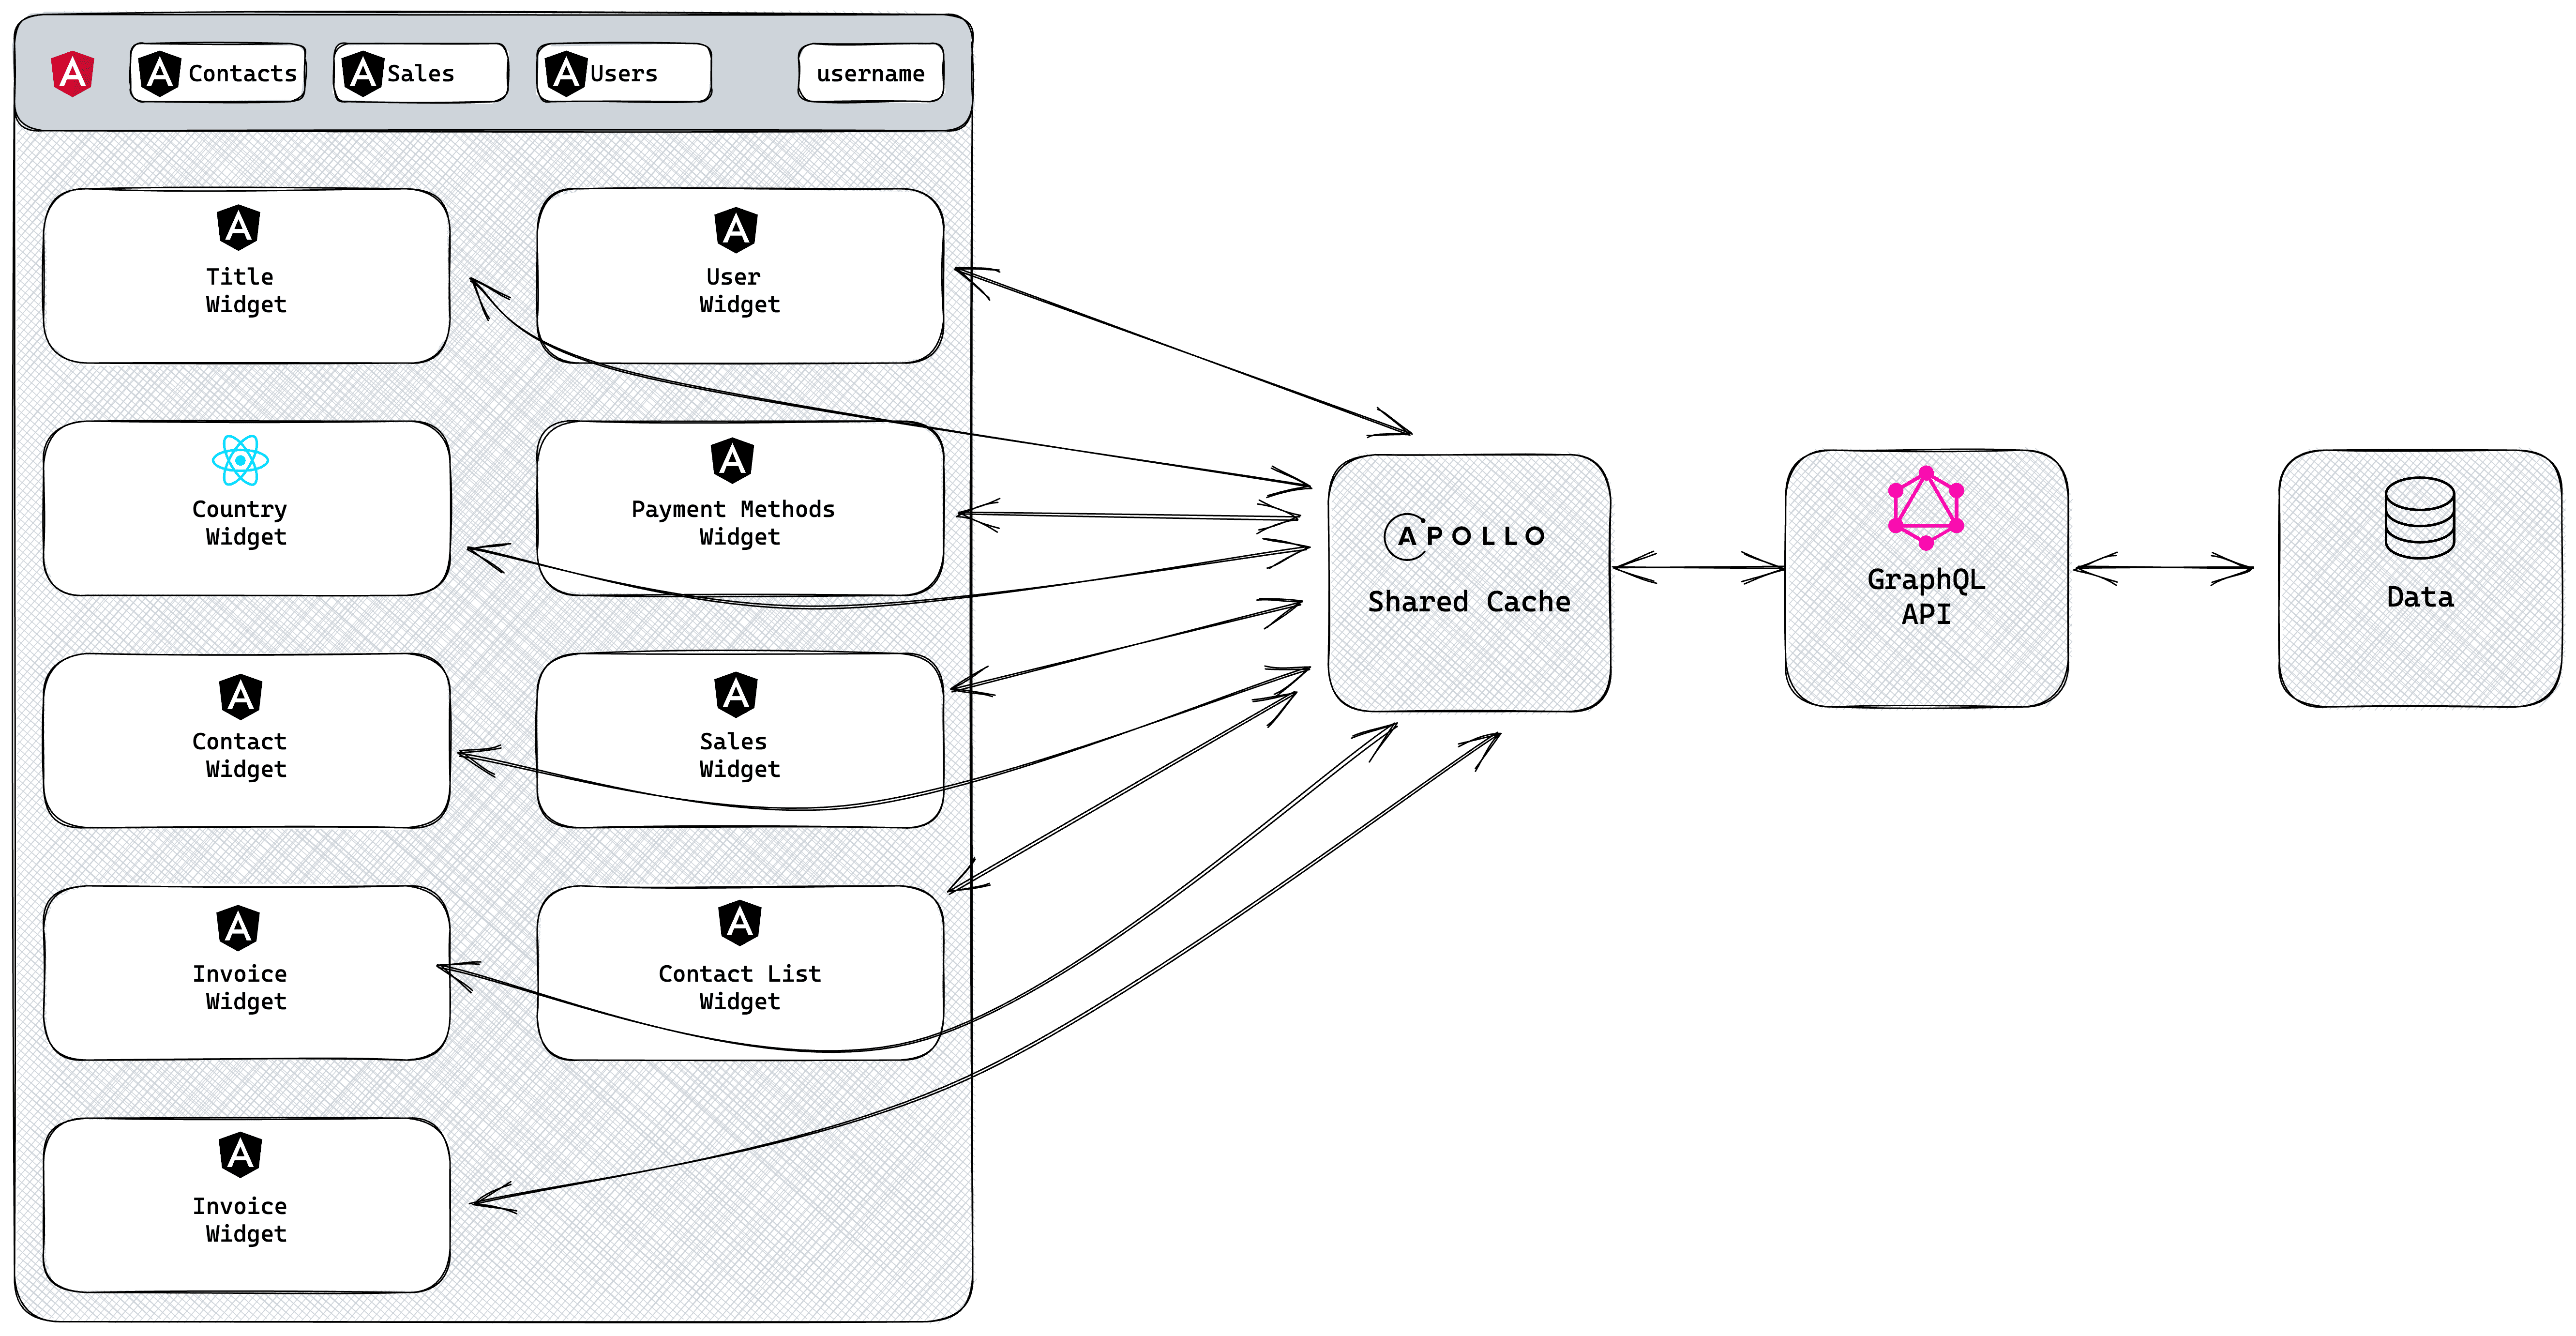
\includegraphics[width=1\linewidth]{images/applied-methods/prototypical-implementation/host-architecture.png}
  \caption{The structure of the micro-frontend prototype.}\label{fig:applied-methods:prototype-micro-frontend-architecture}
\end{figure}
\fi

\noindent Each micro-frontend is deployed separately and is accessible by a separate \ac{URL}. The application shell is the entry point for the client, and it consumes the Dashboard, Contact, Sales, and User application. The main functionality of the micro-frontends is encapsulated in modules. These modules of the applications can be easily accessed through the Module Federation and used by the application shell. The modules are used in exactly the same way in the standalone application.

\bigskip

\noindent The Listing \ref{code:applied-methods:module-federation-config-expose} shows the configuration of the contact micro-frontend to expose its primary implementation through module federation in the form of the \texttt{entry.module}. The configuration of the other micro-frontends looks similar. The properties of the module-federation plugin were already discussed in Section \ref{subsection:background:micro-frontend:module-federation}. All Angular- and Apollo- dependencies are specified to be shared across all micro-frontends. Sharing the dependencies ensures that all micro-frontends use the same and only one version of the dependencies. Listing \ref{code:applied-methods:module-federation-config-expose}, the versions of the dependencies are explicitly specified. Inside the prototype, the versions are read from the root \texttt{package.json} to ensure consistency with the installed versions.

\ifshowListings
\begin{listing}[H]
  \begin{minted}{typescript}
module.exports = {
  name: 'contact',
  exposes: {
    './Module': 'apps/contact/src/app/remote-entry/entry.module.ts',
  },
  shared: [
    '@angular/core': {
      singleton: true, strictVersion: true, requiredVersion: '^15.1.1' 
    },
    ...
    'apollo-angular': { 
      singleton: true, strictVersion: true, requiredVersion: '^4.0.1' 
    },
    ...
  ]
};
  \end{minted}
  \caption{The Module Federation configuration to expose the contact's functionality.}\label{code:applied-methods:module-federation-config-expose}
\end{listing}
\fi

\noindent The application shell is configured to consume the remote modules listed inside the \texttt{remotes}-object. The configuration to consume the four micro-frontends of the architecture can be seen in the Listing \ref{code:applied-methods:module-federation-config-consume}. This configuration allows the application shell to consume the \texttt{entry.module} of the micro-frontend, which was exposed before with the configuration from Listing \ref{code:applied-methods:module-federation-config-expose}. As with the remote module configuration, the application shell shares the same dependencies. Dependency sharing is required so that micro-frontends can load their runtime dependencies from the application shell and use the same dependency version.

\ifshowListings
\begin{listing}[H]
  \begin{minted}{typescript}
module.exports = {
  name: 'host',
  remotes: {
    contact: 'contact@http://localhost:4201/remoteEntry.js'
    sales: 'sales@http://localhost:4202/remoteEntry.js'
    dashboard: 'dashboard@http://localhost:4203/remoteEntry.js'
    user: 'user@http://localhost:4204/remoteEntry.js'
  },
  shared: {
    '@angular/core': {
      singleton: true, strictVersion: true, requiredVersion: '^15.1.1' 
    },
    ...
    'apollo-angular': { 
      singleton: true, strictVersion: true, requiredVersion: '^4.0.1' 
    },
    ...
  }
};
  \end{minted}
  \caption{The configuration of the application shell to be able to consume micro-frontends.}\label{code:applied-methods:module-federation-config-consume}
\end{listing}
\fi

\noindent Using the Module Federation configuration from Listing \ref{code:applied-methods:module-federation-config-consume}, the application shell can load and display the remote modules. Listing \ref{code:applied-methods:angular-route-to-remote-module} shows the route configuration for displaying the contact micro-frontend using Angular's router. Nx offers helper methods like \texttt{loadRemoteModule} for Module Federation to load remote modules into a route of the application shell. The application shell follows the approach of showing one micro-frontend per route. The dashboard on the other hand displays multiple micro-frontend widgets on a page.

\ifshowListings
\begin{listing}[H]
  \begin{minted}{typescript}
const routes: Routes = [
  {
    path: 'contact',
    loadChildren: () => loadRemoteModule('contact', './Module')
      .then((m) => m.ContactRemoteEntryModule),
  },
  ...
]
  \end{minted}
  \caption{An Angular route to the contact application.}\label{code:applied-methods:angular-route-to-remote-module}
\end{listing}
\fi

\ifshowAppliedMethodsCustomNginxConfSection
  \subsection{Deployment problems}\label{subsection:applied-methods:prototypical-implementation:nginx-problems}

Docker is used to run the micro-frontends in production. The Nginx web server in a Docker container is used to deliver the application files to the client. The dockerfile for the micro-frontends is shown in Listing \ref{code:applied-methods:prototype-implementation-dockerfile}. The application to deploy needs to be built before creating the docker image. Afterwards the necessary files are copied into the docker image.

\ifshowListings
  \begin{listing}[H]
  \begin{minted}{dockerfile}
FROM nginx:alpine
COPY nginx/nginx.conf /etc/nginx/nginx.conf
COPY dist/apps/contact/ /usr/share/nginx/html/
    
CMD [
  "/bin/sh", 
  "-c", 
  "envsubst < /usr/share/nginx/html/assets/settings.template.json >" 
  "/usr/share/nginx/html/assets/settings.json && exec nginx -g daemon off;"
]
  \end{minted}
  \caption{The dockerfile for containerizing a micro-frontend.}\label{code:applied-methods:prototype-implementation-dockerfile}
  \end{listing}
\fi

\noindent Module Federation applications expose a file called \texttt{remoteEntry.mjs}, which is consumed by an application shell. However, Nginx currently cannot interpret the mime-type of \texttt{\*.mjs} files which would be \ac{JS}. Therefore, it falls back to the default mime-type \texttt{text/plain}, where \ac{JS} is not executed in the browser. As a workaround for this problem, a custom \texttt{nginx.conf} has been created that sets the default mime-type to \texttt{text/javascript}, which allows the execution of the script in the browser. A part of the configuration is shown in Listing \ref{code:applied-methods:prototype-implementation-custom-nginx-conf}.

\ifshowListings
  \begin{listing}[H]
  \begin{minted}{bash}
default_type text/javascript;
  \end{minted}
  \caption{The custom configuration for Nginx to set the default mime type.}\label{code:applied-methods:prototype-implementation-custom-nginx-conf}
  \end{listing}
\fi

\noindent The custom configuration allows Nginx to correctly load and interpret the remote module files. Setting another default mime type will not break the web server because modern frameworks like Angular just work with \ac{JS} files.

\fi

\subsection{Integrating the React micro-frontend}\label{subsection:applied-methods:prototypical-implementation:react-micro-frontend}

One widget for the dashboard micro-frontend was implemented using the popular frontend framework React. Implementing one micro-frontend in another technology was done to show that the concept of sharing a single cache instance between multiple micro-frontends is technology agnostic. The React widget exposes its functionality like the Angular counterparts through Module Federation. In comparison to Angular, React does not have the concept of modules. Therefore, the functionality of the widget is exported as a simple, functional React component, as shown in listing  \ref{code:applied-methods:module-federation-react-config-expose}.

\ifshowListings
\begin{listing}[H]
    \begin{minted}{typescript}
module.exports = {
  name: 'react-dashboard',
  exposes: { './Module': './src/remote-entry.ts' },
  shared: [
    react: {
      singleton: true, strictVersion: true, requiredVersion: '^18.2.0' 
    },
    ...
  ]
};
    \end{minted}
    \caption{Module Federation config for exposing the \texttt{remote.entry} of the React micro-frontend.}\label{code:applied-methods:module-federation-react-config-expose}
\end{listing}
\fi

\noindent The host application can consume the React application in the same way as the Angular remote modules. However, rendering a React component in an Angular application is natively impossible. Therefore, an Angular wrapper component loads the React remote bundle and renders it inside an HTMLElement. The Angular adapter makes it possible for the Angular router to point to the component, which is impossible with the React component directly.

\bigskip

\noindent Angular modules consumed through Module Federation can access the \ac{DI} tree from the application shell. However, React does not offer a \ac{DI} system like Angular and cannot access the necessary dependencies. React uses contexts to pass down data through the component tree without manually passing properties down level by level. It enables data sharing between components not directly connected in the component tree. The make the shared caching layer inside the React application work, the React widget needs the \texttt{InMemoryCache} instance from the application shell. The shared caching layer is explained in Section \ref{section:applied-methods:shared-caching-layer} in more detail, but the general concept is needed to understand the need to incorporate the instance into the React context. Therefore, the Angular wrapper creates the exposed widget inside a React context provider with the necessary dependencies. The function in listing \ref{code:applied-methods:prototypical-implementation:render-react-component-with-context} shows the React context provider's creation and the React component's rendering. 

\ifshowListings
\begin{listing}[H]
    \begin{minted}{typescript}
render<Comp extends ElementType>(rootEl: Root, Comp: Comp) {
  rootEl.render(
    createElement(
      NgReactContext, {
        ctx: {
          graphQLClientCache: this.injector.get(GRAPHQL_CLIENT_CACHE),
          ...
        },
      },
      createElement(Comp, compProps)
    )
  );
}
    \end{minted}
    \caption{The function to render the React widget into an Angular component.}\label{code:applied-methods:prototypical-implementation:render-react-component-with-context}
\end{listing}
\fi

\noindent With the help of the function, the widget can access the instance of the \texttt{InMemoryCache} from the application shell and use it to share the cache between the Angular and the React micro-frontend. How the \texttt{InMemoryCache} from the application shell is injected and consumed is shown in listing \ref{code:applied-methods:prototypical-implementation:consume-react-context}. The cache is used to create a new instance of the ApolloClient, and afterwards the client is provided to the application using another context.

\ifshowListings
\begin{listing}[H]
    \begin{minted}{typescript}
const injector = useContext(InjectorCtx);

const client = new ApolloClient({
  uri: injector.graphQLEndpoint,
  cache: injector.graphQLClientCache,
  ...
});

return (
  <ApolloProvider client={client}>
    <PaymentMethodList />
  </ApolloProvider>
);

    \end{minted}
    \caption{Use the \texttt{InMemoryCache} instance from the React context.}\label{code:applied-methods:prototypical-implementation:consume-react-context}
\end{listing}
\fi


\subsection{Backend for frontend}\label{subsection:background:prototypical-implemenation:bff}

The \ac{BFF} pattern was implemented using GraphQL. A single \ac{BFF} service is used for all micro-frontends of the architecture. Apollo Server is used as the GraphQL server and was chosen to implement the \ac{API}. Every micro-frontend uses the same \ac{BFF} service, however, multiple GraphQL \acp{API} could be used. Each micro-frontend is a standalone application, therefore it could communicate with multiple GraphQL \acp{API}.
The GraphQL \ac{API} fetches the data from a cluster of microservices and brings the results into the correct shape for the micro-frontends. The GraphQL \ac{API} was developed, while the microservices were still under development. However, the data model was already finalized. Therefore, the GraphQL \ac{API} was implemented using mock data. The mock data was generated using the database schemas of the microservices. The queries and mutations were implemented by directly reading and writing the mock data. Once the microservices are implemented, the GraphQL \ac{API} will be modified to communicate directly with the microservices within the company.


\ifshowAppliedMethodsLoadRemoteSettingsSection
  \subsection{Remote application configuration}\label{subsection:applied-methods:prototypical-implementation
:load-remote-settings}

The application shell is set up to use dynamic Module Federation. The location of the remote applications is determined at runtime. The problem with the so-called static Module Federation is that the \ac{URL} of the remote application must be known at build time. However, this is troublesome if the application should be built once and deployed to multiple stages. It is very cumbersome to build an artifact for every environment.

\bigskip

\noindent One possibility to fetch the remote definitions at runtime is to store them in a simple \ac{JSON} file, which can easily be configured for every environment. The host makes a simple GET request to get the definitions inside the \ac{JSON} file. The content of the file has to be a simple mapping between the name of the remote and their location, as shown in Listing \ref{code:applied-methods:define-module-federation-manifest}.

\ifshowListings
\begin{listing}[H]
\begin{minted}{json}
{
  "sales": "http://localhost:4201",
  "contact": "http://localhost:4202",
  "dashboard": "http://localhost:4203",
  "user": "http://localhost:4204"
}
\end{minted}
\caption{The structure of the micro-frontend definition file with the name and \ac{URL}.}\label{code:applied-methods:define-module-federation-manifest}
\end{listing}
\fi

\noindent The host has to fetch the definitions when starting up the application. The definitions are stored and stored for the Webpack configuration, as shown in Listing \ref{code:applied-methods:load-module-federation-settings}. If the file can be fetched successfully, the bootstrap process of the application gets imported dynamically.

\ifshowListings
\begin{listing}[H]
\begin{minted}{typescript}
fetch('/assets/module-federation.manifest.json')
  .then((res) => res.json())
  .then((definitions) => setRemoteDefinitions(definitions))
  .then(() => import('./bootstrap').catch((err) => console.error(err)));
\end{minted}
\caption{Loading the micro-frontend definition file during initialization.}\label{code:applied-methods:load-module-federation-settings}
\end{listing}
\fi

\noindent Another use case for dynamic content is the configuration of an application. This configuration includes the endpoint of the GraphQL \ac{API}, which can be different in staging and production. Therefore, the configuration should also be fetched dynamically. The settings are fetched during the first load of the application and stored for later use. The configuration is stored inside a file called \texttt{settings.json}, served alongside the application. Angular provides a handy mechanism to run code when the application is loaded.

\bigskip

\noindent With the help of the \texttt{APP\_INITIALIZER} injection token, asynchronous code can be executed when the application starts up. Such tasks include fetching data from a remote \ac{API} and setting up configuration or initializing third-party libraries. When an Angular app starts, it will execute all the functions registered with \texttt{APP\_INITIALIZER} in the order they were defined. If one of the initialization tasks fails, the application will not load. \cite{misc:-:applied-methods:prototype-implementation:angular-app-initializer}

\bigskip

\noindent The Listing \ref{code:applied-methods:fetch-and-store-settings} shows a simplified version to fetch and store the settings in the local storage. The settings are fetched from the \texttt{settings.json} file, which content is used to configure the application. The settings of the application shell are stored with the key \texttt{host}. Each application of the micro-frontend architecture stores its settings with its application name as the key.

\ifshowListings
\begin{listing}[H]
\begin{minted}{typescript}
@NgModule({
  providers: [{
    provide: APP_INITIALIZER,
    async useFactory(http: HttpClient, storage: StorageClient) {
      const environmentConfig = await lastValueFrom(
        http.get('assets/settings.json')
      );
      storage.store('host', environmentConfig);
    },
    multi: true,
    deps: [HttpClient, StorageClient],
  }]
})
class CoreModule {}
\end{minted}
\caption{Fetch \& store the settings of the application shell.}\label{code:applied-methods:fetch-and-store-settings}
\end{listing}
\fi

\subsubsection{Loading the configuration of the remote applications}\label{subsubsection:applied-methods:prototypical-implementation
:load-the-configuration}

Each application of the prototypical micro-frontend architecture follows this approach. When the application is initialized, the application configuration is fetched with a GET request from the \texttt{settings.json}. As mentioned in the previous section, each micro-frontend stores its settings with the application's name as the key. However, the configuration does not get fetched when the application shell consumes the functionality of a micro-frontend. Therefore, the application throws errors because they cannot access their settings from the storage. To solve the problem of missing settings for the application, the configuration of a remote application is fetched and stored inside a store when the user navigates to it. This procedure is explained visually in Figure \ref{fig:applied-methods:load-remote-settings}.

\ifshowImages
  \begin{figure}[H]
  \centering
  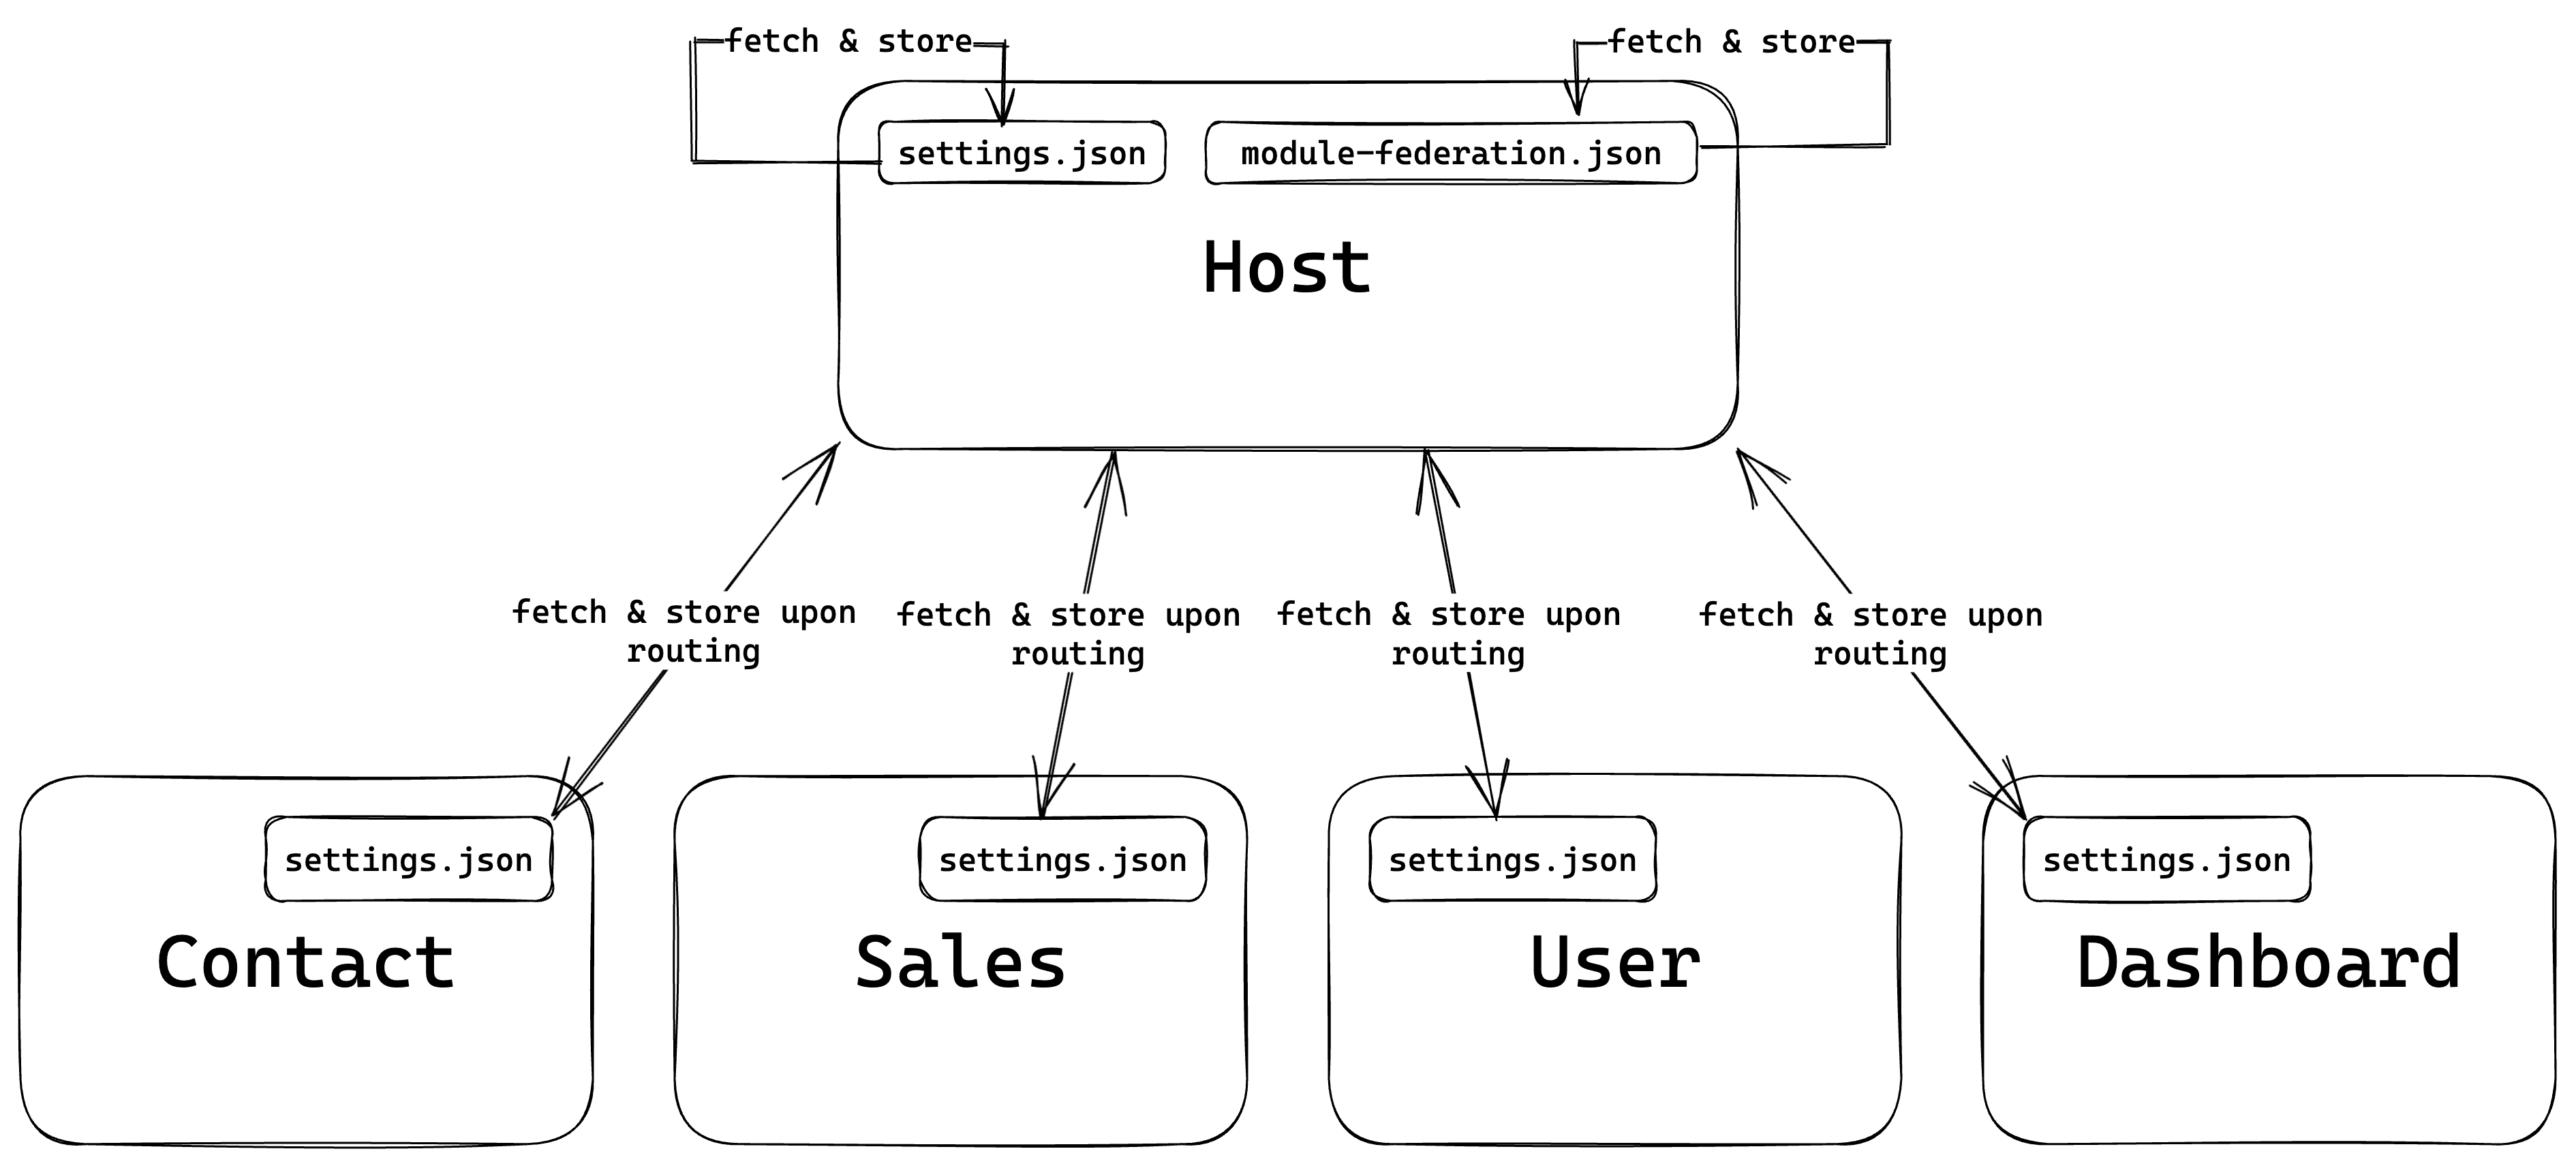
\includegraphics[width=0.9\linewidth]{images/applied-methods/prototypical-implementation/load-remote-settings.png}
  \caption{Loading a storing the configuration of the remote applications.}\label{fig:applied-methods:load-remote-settings}
  \end{figure}
\fi

\noindent With the help of Angular resolvers, the resolvers executed before the components of the target are rendered. Due to the dynamic Module Federation, the location of the remote module is known. Therefore, the \texttt{settings.json} is loaded and stored in addition to loading the remote module. A simplified version of the code is shown in Listing \ref{code:applied-methods:fetch-and-store-remote-application-settings}. The same principle applies to every remote module, which is consumed.

\ifshowListings
\begin{listing}[H]
\begin{minted}{typescript}
const routes: Routes = [{
    path: 'contact',
    loadChildren: () => loadRemoteModule('contact', './Module')
      .then((m) => m.ContactRemoteEntryModule),
    resolve: {
      settings: () => {
        const contact = inject(StorageClient).get('manifest')['contact'];
        return inject(HttpClient).get(`\${contact}/assets/settings.json`);
      }
    },
  },
  ...
]
\end{minted}
\caption{Fetch the settings of the contact application.}\label{code:applied-methods:fetch-and-store-remote-application-settings}
\end{listing}
\fi

\noindent With this approach, each application can access its settings like running in standalone mode. Moreover, it has another benefit because each application can only access its settings and not the settings of the other applications. 

\fi

\ifshowAppliedMethodsSecondaryEntrypoints
  \subsection{Sharing secondary entry points}\label{subsection:applied-methods:prototypical-implementation:sharing
-secondary-entrypoints}

By default, all dependencies of the micro-frontends are shared through Module Federation. The configuration options for every dependency are \texttt{singleton}-, \texttt{strictVersion}-, and \texttt{requiredVersion}-property. These properties are explained in more detail in Section \ref{subsection:background:micro-frontend:module-federation}. The versions of these dependencies are determined automatically from the \texttt{package.json}. However, not all packages support being shared with these default settings. The npm package \texttt{@apollo/client} has a problem because it has secondary entry points. When trying to share \texttt{@apollo/client/core}, \texttt{@apollo/client/link/batch} and \texttt{@apollo/client/link/error} the error message in Figure \ref{fig:applied-methods:sharing-secondary-entrypoints-error} is shown.

\ifshowImages
  \begin{figure}[H]
  \centering
  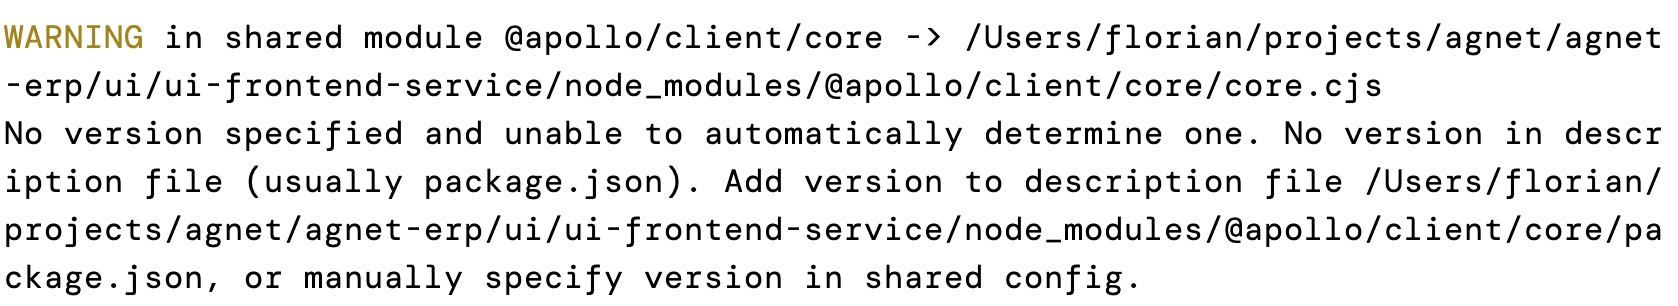
\includegraphics[width=1\linewidth]{images/applied-methods/prototypical-implementation/module-federation-apollo-warning.jpg}
  \caption{A Module Federation warning, when the dependency \texttt{@apollo/client} should be shared.}\label{fig:applied-methods:sharing-secondary-entrypoints-error}
  \end{figure}
\fi

\noindent The problems are secondary entry points like \texttt{@apollo/client/core}, which are a bit like an npm package in another npm package. The \texttt{package.json} of \texttt{@apollo/client/core} is shown in Listing \ref{code:applied-methods:package-json-apollo-client-core}. Webpack tries to resolve the version of the secondary entry point from the \texttt{package.json} and not from \texttt{@apollo/client}. Therefore, it cannot determine the version and prints the warning shown in Figure \ref{fig:applied-methods:sharing-secondary-entrypoints-error}. The warning does not lead to an error, but these dependencies cannot be shared and must be included in every micro-frontend bundle.

\ifshowListings
\begin{listing}[H]
  \begin{minted}{json}
{
  "name": "@apollo/client/core",
  "type": "module",
  "main": "error.cjs",
  "module": "index.js",
  "types": "index.d.ts",
  "sideEffects": false
}
  \end{minted}
  \caption{The \texttt{package.json} of \texttt{@apollo/client/core}.}\label{code:applied-methods:package-json-apollo-client-core}
\end{listing}
\fi

\noindent The Module Federation was fixed by specifying the version for these packages manually. The version is the same as that of \texttt{@apollo/client}. The configuration for the sharing of these packages is shown in the Listing \ref{code:applied-methods:sharing-secondary-entrypoints-config}. 

\ifshowListings
\begin{listing}[H]
  \begin{minted}{typescript}
shared: (libraryName, defaultConfig) => {
  if (libraryName.includes(`@apollo/client/`))
    return { ...defaultConfig, version: '^3.6.9' };

  return defaultConfig;
}
  \end{minted}
  \caption{Specify the version for the secondary entry points for the \texttt{@apollo/client} package.}\label{code:applied-methods:sharing-secondary-entrypoints-config}
\end{listing}
\fi

\fi
\section{Communication from the shell- to the remote-application}\label{section:methods:communication-shell-remote}

To solve the problem of building a common caching layer, some form of communication between the shell and remote application had to be implemented. To ensure that the micro-frontends remain independent of each other, it should be avoided that they communicate directly with each other.

Angular provides a great tool for this use case, namely dependency injection. The shell application can provide services that can later be injected by the remote applications. This is very handy because the micro frontend can provide the same services as the shell application in standalone mode. Therefore, the remote module can be easily used within the remote and shell application.

For example i implemented a layout-service that takes advantage of dependency injection.

\ifshowImages
\begin{figure}[H]
\centering

\includegraphics[width=1\linewidth]{images/prototype-screenshots/contact-header.png}
\caption{Beispiel für die Beschriftung eines Buchrückens.}
\end{figure}
\fi

\ifshowImages
\begin{figure}[H]
\centering

\includegraphics[width=1\linewidth]{images/prototype-screenshots/host-contact-header.png}
\caption{Beispiel für die Beschriftung eines Buchrückens.}
\end{figure}
\fi

\section{Shared caching layer}\label{section:applied-methods:shared-caching-layer}

The previous section explained how the communication strategy within the micro-frontend architecture works behind the scenes. Apollo Client's caching mechanism should be used to boost the performance of the micro-frontend architecture and handle the problems of over-fetching and over-requesting. This section goes into more detail, how the shared caching layer is implemented and integrated into the architecture. The structure of the shared caching layer is shown in Figure \ref{fig:applied-methods:structure-shared-caching-layer}. Each micro-frontend has a separate instance of the Apollo Client, but they should all use the same instance of the \texttt{InMemoryCache}. Therefore, each application can provide its own configuration for the Apollo Client, however all micro-frontend use the same instance of the \texttt{InMemoryCache}. The \texttt{InMemoryCache} stores the results of GraphQL queries. When a micro frontend needs to retrieve a query that is already cached, it can reuse the data that is already cached instead of retrieving it again from the GraphQL \ac{API} again. This caching strategy reduces the number of network requests and thus the amount of data that has to be transferred over the network.

\ifshowImages
  \begin{figure}[H]
  \centering
  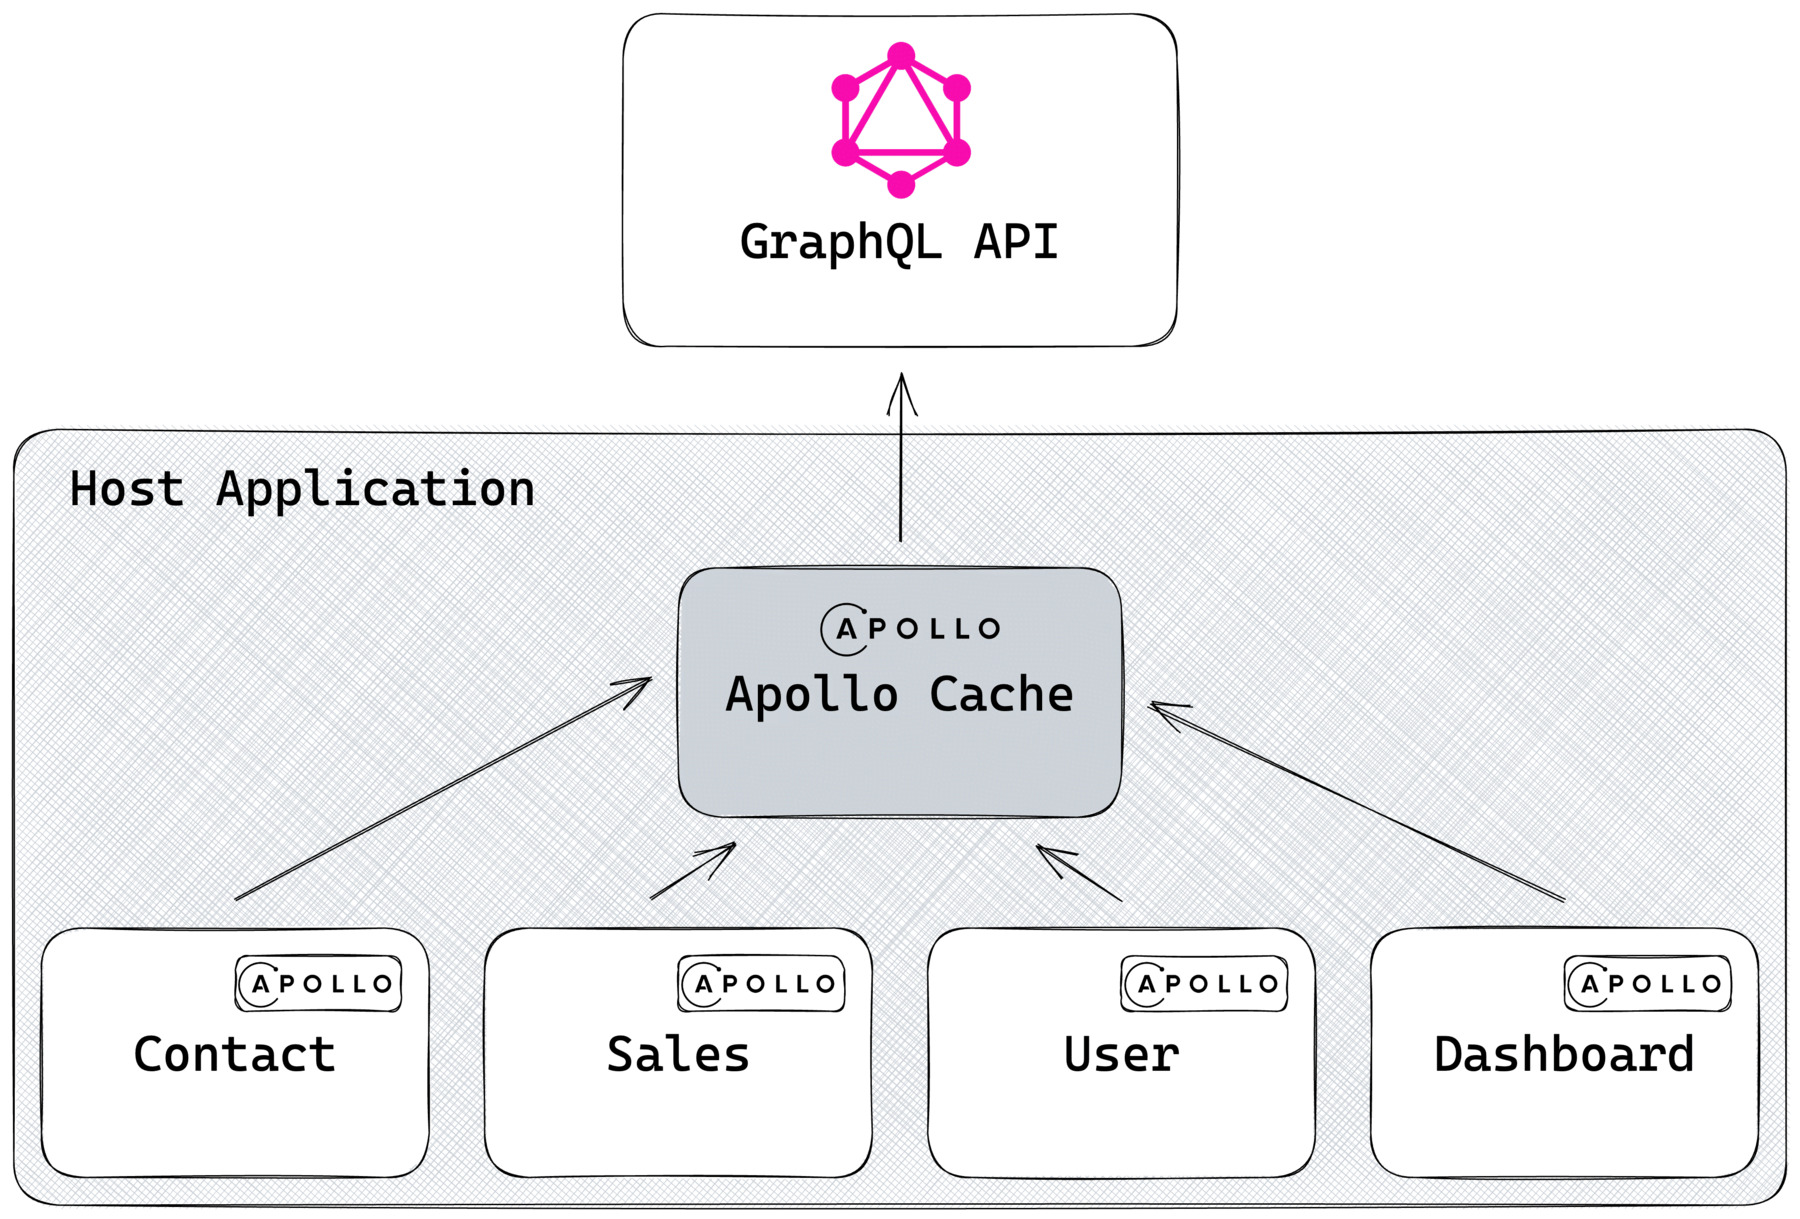
\includegraphics[width=0.7\linewidth]{images/applied-methods/shared-caching-layer/shared-caching-layer.jpg}
  \caption{The structure of the shared caching layer.}\label{fig:applied-methods:structure-shared-caching-layer}
  \end{figure}
\fi

\noindent The application shell must provide the instance of the GraphQL \texttt{InMemoryCache} to make sure that all micro-frontends have the same instance. Listing \ref{code:applied-methods:creating-the-apollo-client} shows how the Apollo Client is created for an Angular application with default settings. The \texttt{cache} property is important, as it needs an instance of Apollo's \texttt{InMemoryCache}. This allows for the architecture to create a single cache instance elsewhere and pass it to the Apollo Client. 

\ifshowListings
\begin{listing}[H]
\begin{minted}{typescript}
@NgModule({
  imports: [ApolloModule],
  providers: [{
    provide: APOLLO_OPTIONS,
    useFactory: (httpLink: HttpLink) => ({
      cache: new InMemoryCache(),
      link: httpLink.create({ uri: 'http://localhost:3000' }),
    }),
    deps: [HttpLink],
  }]
})
class AppModule {}
\end{minted}
\caption{Create a new instance of the Apollo Client.}\label{code:applied-methods:creating-the-apollo-client}
\end{listing}
\fi

\noindent The concept behind the shared caching layer is to instantiate the cache instance inside the application shell and provide it to the micro-frontends. The instance of the \texttt{InMemoryCache} should be injectable through an injection token, just like the injection token from Section \ref{section:applied-methods:communication-shell-remote}, which specifies whether the application runs in standalone mode. The injection token can be provided by the application shell and injected and used by the micro-frontends. Moreover, the application itself can provide the instance of the cache when it runs in standalone mode. The \texttt{GRAPHQL\_CLIENT\_CACHE} token can be used to provide an instance of Apollo's \texttt{InMemoryCache} to the micro-frontends, as shown in Listing \ref{code:applied-methods:graphql-client-cache-provider}.

\ifshowListings
\begin{listing}[H]
\begin{minted}{typescript}
@NgModule({
  providers: [
    { provide: GRAPHQL_CLIENT_CACHE, useValue: new InMemoryCache() }
  ]
})
class HostCoreModule {}
\end{minted}
\caption{Provide the instance of the \texttt{InMemoryCache} to \ac{DI}.}\label{code:applied-methods:graphql-client-cache-provider}
\end{listing}
\fi

\subsection{GraphQL Client creation}{subsection:applied-methods:shared-caching-layer:graphql-client-creation}

\noindent The prototype provides abstractions to create the necessary configuration for using the Apollo Client more easily and identically for all micro-frontends. Listing \ref{code:applied-methods:graphql-client-creation} shows the usage of the abstraction to create a new instance of Apollo Client for a micro-frontend. The module \texttt{GraphQLClientOptionsModule} hides the complexity of creating and providing a Apollo Client instance, as shown in Listing \ref{code:applied-methods:creating-the-apollo-client-with-a-shared-cache}. The moduls has a required parameter that specifies a unique name. This name is used to identify and track active Apollo Clients inside the architecture. The \texttt{GraphQLClientOptionsModule} should be used in every module that needs GraphQL functionality and is exposed through Module Federation. When the micro-frontend is then integrated within the application shell, it has its own instance of the Apollo Client. This facilitates independent development of micro-frontends, as the Apollo Client configuration remain the same whether it is running in standalone mode or consumed by the application shell. For example, a problem could arise if the application shell provides the instance of the Apollo Client and the contact micro-frontend injects that instance with \ac{DI}. The contact development team might configure the Apollo Client differently within the contact application, and the functionality might not work as expected within the application-shell because the configuration might be different.

\ifshowListings
  \begin{listing}[H]
    \begin{minted}{typescript}
@NgModule({
  imports: [ GraphQLClientOptionsModule.withConfig('contact-remote') ]
})
class ContactRemoteCoreModule {}
  \end{minted}
  \caption{Create the Apollo Client instance for the micro-frontend.}\label{code:applied-methods:graphql-client-creation}
  \end{listing}
\fi

\ifshowListings
\begin{listing}[H]
\begin{minted}{typescript}
@NgModule({
  imports: [ApolloModule],
  providers: [{
    provide: APOLLO_OPTIONS,
    useFactory(httpLink: HttpLink, cache: InMemoryCache) {
      const link = httpLink.create({uri: 'http://localhost:3000'});
      return { cache, link };
    },
    deps: [HttpLink, GRAPHQL_CLIENT_CACHE],
  }]
})
class ContactRemoteModule {}
\end{minted}
\caption{Access the shared \texttt{InMemoryCache} instance from \ac{DI}.}\label{code:applied-methods:creating-the-apollo-client-with-a-shared-cache}
\end{listing}
\fi

\noindent The \texttt{GraphQLClientOptionsModule} uses the storage service to get the required configuration for the Apollo Client. For example, \ac{URL} of GraphQL \ac{API} is taken from the storage service. By default, it tries to inject the \texttt{GRAPHQL\_CLIENT\_CACHE}, and use it as the cache instance for the Apollo Client. If it cannot be injected, a separate cache instance is created for the client. An addtional injection token \texttt{GRAPHQL\_CLIENT\_OPTIONS\_CONFIG} can be used to specify additional options for creating a new Apollo Client instance. The injection token's usage and default options are shown inside Listing \ref{code:applied-methods:graphql-client-extra-configuration-options}. The injection token must be provided inside the same module where the \texttt{GraphQLClientOptionsModule} was defined.

\ifshowListings
\begin{listing}[H]
\begin{minted}{typescript}
@NgModule({
  providers: [{
    provide: GRAPHQL_CLIENT_OPTIONS_CONFIG,
    useValue: {
      shareCache: true,
      persistCache: false,
      useTypePolicies: true,
      typePolicies: CONTACT_TYPE_POLICIES,
    },
  }]
})
class ContactRemoteCoreModule {}
\end{minted}
\caption{Provide additional options for creating the Apollo Client instance.}\label{code:applied-methods:graphql-client-extra-configuration-options}
\end{listing}
\fi

\noindent The options include \texttt{shareCache}, \texttt{persistCache}, \texttt{useTypePolicies} and \texttt{typePolicies}. The \texttt{shareCache} setting is used to specify whether the Apollo Client should use the \texttt{InMemoryCache} instance provided by \texttt{GRAPHQL\_CLIENT\_CACHE} or if it should create a new instance, specifically for this remote module. The \texttt{persistCache} option is set to \texttt{false} by default. It stores the contents of the \texttt{InMemoryCache} inside the \texttt{localStorage}. This feature provided by the Apollo Client allows faster initial page renders, because the data from the \texttt{localStorage} is transferred back to the cache when the application is loaded. The options \texttt{useTypePolicies} and \texttt{typePolicies} are used together and must be specified together. The property \texttt{useTypePolicies} specifies whether the type policies from the option \texttt{typePolicies} should be used or not. Type policies allow Apollo Client to customize the read and write operations of every field inside the cache. They are explained in more detail in Section \ref{subsubsection:background:graphql:apollo-server-client:type-policies}. As explained earlier, each micro-frontend has its own Apollo client instance with a shared cache instance, so the type policies cannot be registered directly when the \texttt{InMemoryCache} is created. The option \texttt{typePolicies} has the same type as the \texttt{typePolicies} parameter of the \texttt{InMemoryCache} constructor. Specifying the option when providing the \texttt{GRAPHQL\_CLIENT\_OPTIONS\_CONFIG} allows the micro-frontend to specify additional type policies for the cache. Part of the code to create the shared cache and append type-policies within the \texttt{GraphQLClientOptionsModule} is shown in Listing \ref{code:applied-methods:adding-extra-type-policies}. First, the instance of the cache should be injected. If the cache cannot be injected, it means that the Apollo Client has to create a new instance of the \texttt{InMemoryCache}. The \texttt{typePolicies} are added to the cache instnace if both options \texttt{typePolicies} and \texttt{useTypePolicies} are truthy values.

\ifshowListings
\begin{listing}[H]
\begin{minted}{typescript}
const cache = inject(GRAPHQL_CLIENT_CACHE, { optional: true });
const { shareCache, useTypePolicies, typePolicies } = graphQLClientOptions;

const cacheInstance = shareCache ? cache : new InMemoryCache();

if (typePolicies && useTypePolicies)
  clientCache.policies.addTypePolicies(typePolicies);
\end{minted}
\caption{Insert additional type policies into the cache instance.}\label{code:applied-methods:adding-extra-type-policies}
\end{listing}
\fi

\section{Built a mechanism that reduces the size of queries}\label{section:applied-methods:query-reduction}

After implementing the shared caching layer, the next step was to improve the performance of the micro-frontends by optimizing the use of the cache. The size of the network requests can be reduced by removing parts of a query that are already inside the cache. The theory behind removing fields from the query was already explained in Section \ref{subsection:background:graphql:query-reduction}. The Apollo Client does not provide such a functionality out of the box, but many users request the feature in Apollo's Github Repository. Section \ref{subsubsection:background:graphql:apollo-server-client:in-memory-cache-working} explains how the \texttt{InMemoryCache} of Apollo Client works in more detail. Briefly summarized the caching works with the name and the parameters of a GraphQL query. For example, if a query is executed against the GraphQL \ac{API}, the results of the query are cached. If the same query with the same fields is executed again with the same parameters, the results are fetched from the Apollo Client cache. If the query fetches an additional field, not inside the cache, the complete query is sent to the GraphQL \ac{API}. Only if the queried fields are identical the cache data is used. Consequently, identical queries that fetch different fields are always fetched from the server.

\bigskip

\noindent Consider Listing \ref{code:applied-methods:compare-allusers-user-query}, where the left query fetches all users, and the query on the right fetches a user by its id. Both queries fetch the same data type and the same fields, but they are fundamentally different queries. They have different names and different parameters. Both queries are sent to the GraphQL \ac{API}. The query on the right could be omitted if the user with the given id is fetched from the cache. If the left query is executed before the query on the right, the data to resolve the query on the right could be taken entirely from the cache.

\ifshowListings
\begin{listing}[H]
\begin{minted}{typescript}
query allUsers {                        query user(id: ID!) {
  allUsers {                              user(id: \$id) {
    id                                      id
    username                                username
    email                                   email
    firstName                               firstName
    secondName                              secondName
  }                                       }
}                                      }
\end{minted}
\caption{Comparison between the \texttt{allUsers} and \texttt{User} query.}\label{code:applied-methods:compare-allusers-user-query}
\end{listing}
\fi

\noindent Apollo offers a solution to tackle this problem. The application might have a detail view and a list view that query the same data as in Listing \ref{code:applied-methods:compare-allusers-user-query}. The user query data might already be in the cache, but the Apollo Client does not know that. Therefore, the cache lookup can be configured so the Apollo Client knows where to look for the data. A basic understanding of type policies is needed to understand the cache redirection, described in more detail in Section \ref{subsubsection:background:graphql:apollo-server-client:type-policies}.

\bigskip

\noindent A field policy \texttt{read} function must be written for the user query to inform the Apollo Client where to look for the cached \texttt{User} object. Like the \texttt{firstName} being a \texttt{User} type field, the user query is a field of the root query. This hierarchy resembles the structure of the GraphQL Schema, where the queries have to be defined inside the \texttt{Query} type. Listing \ref{code:applied-methods:query-reduction:graphql-schema} shows an excerpt from the GraphQL schema. All queries that a client can execute are listed inside the \texttt{Query} type.

\ifshowListings
\begin{listing}[H]
\begin{minted}{typescript}
type Query {
  user(id: ID!): User
  allUsers(page: Int, perPage: Int): [User]
  ...
}

type User {
  id: ID!
  firstName: String!
  secondName: String!
  ...
}
\end{minted}
\caption{An excerpt from the GraphQL schema.}\label{code:applied-methods:query-reduction:graphql-schema}
\end{listing}
\fi


\noindent Listing \ref{code:applied-methods:query-reduction:user-cache-redirect} shows the \texttt{read} field policy for the \texttt{User}. Like in the GraphQL schema from Listing \ref{code:applied-methods:query-reduction:graphql-schema}, the user query is a field of the root query. Therefore, the read function is executed every time the client runs the user query. The \texttt{toReference} function is used to cache a reference for a \texttt{User} type. The reference is generated based on its \texttt{\_\_typename} and \texttt{id}, as explained in Section \ref{subsubsection:background:graphql:apollo-server-client:data-normalization}. Apollo Client uses the result of \texttt{toReference} to look up the object in its cache and return it if it is present. The query is sent to the GraphQL \ac{API} if the object is not in the cache.

\ifshowListings
\begin{listing}[H]
\begin{minted}{typescript}
new ApolloClient({
  cache: new InMemoryCache({ typePolicies: { Query: { fields: {
    User: {
      read(_, { args, toReference }): {
        return toReference({ __typename: 'User', id: args.id });
      }
    }
  }}}})
});
\end{minted}
\caption{Writing a cache-redirect for the User-type.}\label{code:applied-methods:query-reduction:user-cache-redirect}
\end{listing}
\fi

\noindent Using cache redirects to reduce the amount of network requests works, but all of the query's requested fields must be already present in the cache. If the user query fetches any field that the allUsers query did not, Apollo Client considers the cache hit incomplete, and the query is executed over the network. That a detail view and a list view are perfectly identical is very rare in applications. Therefore, this approach cannot effectively reduce the size of network requests. Moreover, the approach is very verbose because a redirect has to be written for every data type. The approach does not scale; the same type-policies must be written and registered for every micro-frontend.

\bigskip

\noindent The open-source project \href{https://github.com/appmotion/apollo-augmented-hooks}{apollo-augmented-hooks} on GitHub provides drop-in replacements for Apollo's GraphQL query methods. It provides the functionality to remove fields from a query already in the cache. However, the big problem is that the project was developed specifically for React's Apollo Client. The dependencies were outdated, and the latest release of the library was in 2021. The library's functionality could only be tested with an old Apollo Client and React version. The dependency offered the functionality to remove fields in the cache from a previous GraphQL query. The Apollo-augmented-hooks dependency was forked to use the functionality of the library inside the prototypical micro-frontend architecture. The first step was to update the dependencies to make it work with the latest version of Apollo Client. The problem with the old implementation is that it just supports React's Apollo Client with its hooks. The core functionality of the library was extracted, and an adapter for React and Angular was written utilizing the functionality. The functions have the same \ac{API} as Apollo's original methods, so migration to the new functions is straightforward. The library's functionality was rewritten with \ac{TS}, adding additional features that utilize the cache even more. The implementation is detailed further in Section \ref{subsection:applied-methods:query-reduction:how-does-the-library-work}.

\ifshowAppliedMethodsTestingQueryReduction
  \subsection{Implementing a query reduction testing layer}\label{subsection:applied-methods:query-reduction:testing-query-reduction}

The following abstraction, seen in Listing \ref{code:applied-methods:query-reduction:graphql-client} for the GraphQL client, was created to compare the Apollo Client's default behavior with the improved behavior of reducing queries.The \texttt{watchQuery} and \texttt{mutate} functions have the same \ac{API} as Apollo Client's original query and mutate functions. Two implementations (\texttt{ReduceGraphQLClientImpl}, \texttt{GraphQLClientImpl}) were created for the base class \texttt{GraphQLClient}. The \texttt{ReduceGraphQLClientImpl} uses query reduction, while \texttt{GraphQLClientImpl} utilizes the original Apollo Client functions. A switch is used to determine which implementation is created at runtime.

\ifshowListings
\begin{listing}[H]
\begin{minted}{typescript}
abstract class GraphQLClient {
  abstract watchQuery<TData, TVariables>(
    options: WatchQueryOptions<TData, TVariables>
  ): Observable<QueryResult<TData>>;

  abstract mutate<TData, TVariables>(
    options: MutationOptions<TData, TVariables>
  ): Observable<MutationResult<TData>>;
}
\end{minted}
\caption{The abstract base class for the GraphQL client.}\label{code:applied-methods:query-reduction:graphql-client}
\end{listing}
\fi

\noindent The switch is implemented as a \ac{DI} token, which can be specified in the applications. The \texttt{REDUCE\_QUERY\_OPTIONS} injection token determines whether the query reduction should be used. The usage of the token is shown in the Listing \ref{code:applied-methods:query-reduction:switch-between-apollo-client-and-query-reduction}. The switch decides whether the \texttt{ReduceGraphQLClientImpl} or \texttt{GraphQLClientImpl} is created. The \texttt{ReduceGraphQLClientImpl} is created when the \texttt{reduceQueries} property is set to \texttt{true}. The provider is specified inside the core module of the application to create the provider globally.

\ifshowListings
\begin{listing}[H]
\begin{minted}{typescript}
const REDUCE_QUERY_OPTIONS = 
  new InjectionToken<ReduceQueryOptions>('reduce-query-options');

@NgModule({
  providers: [{
    provide: REDUCE_QUERY_OPTIONS,
    useValue: { reduceQueries: true },
  }]
})
class ContactCoreModule {}
\end{minted}
\caption{Specify whether queries should be reduced.}\label{code:applied-methods:query-reduction:switch-between-apollo-client-and-query-reduction}
\end{listing}
\fi


\fi

\subsection{Query reduction mechanism}\label{subsection:applied-methods:query-reduction:how-does-the-library-work}

This section briefly describes how the query reduction functionality removes fields from the query using the \texttt{InMemoryCache}. Apollo Client allows specifying multiple configuration options when fetching a query from a GraphQL \ac{API}. Three important options are \texttt{variables}, \texttt{query}, and \texttt{fetchPolicy}. The \texttt{query} specifies the GraphQL query, and the \texttt{variables} are the variables for the query. The fetch policy lets the client specify how data is stored and retrieved from the cache. The typical structure of a GraphQL query inside the micro-frontend architecture is shown in Listing \ref{code:applied-methods:query-reduction:executing-graphql-query}. The query fetches the user's details with the given \texttt{id}. The default fetch policy of a query is \texttt{cache-first}.

\ifshowListings
\begin{listing}[H]
\begin{minted}{typescript}
this.graphQLClient.watchQuery({
  variables: { id: `36bad921-8fcf-4f33-9f29-0d3cd70205c8` },
  query: USER_BY_ID_QUERY,
  fetchPolicy: 'cache-first',
});
\end{minted}
\caption{Defining and running a GraphQL query with Apollo Client.}\label{code:applied-methods:query-reduction:executing-graphql-query}
\end{listing}
\fi

\noindent The Apollo Client offers several fetch policies that customize how the client retrieves data from the cache. The available fetch policies are: \cite{misc:-:applied-methods:query-reduction:apollo-client:queries}

\begin{itemize}
  \item \textbf{cache-first (default)}: This fetch policy instructs the Apollo Client first to check the local cache for the query result. If the data is present in the cache, it is returned immediately. Otherwise, Apollo Client will execute the query and fetch the result from the server, which will then be cached.
  \item \textbf{cache-and-network}: This fetch policy combines the cache-first and network-only policies. Apollo Client first checks the cache for the query result and returns it immediately if it is present. Then, a network request is made to fetch the most up-to-date data, which is then used to update the cache. This fetch policy is a good option for displaying data that gets updated frequently.
  \item \textbf{cache-only}: This fetch policy tells Apollo Client only to check the cache for the query result. If the result is present in the cache, it is returned immediately.
  \item \textbf{network-only}: This fetch policy instructs Apollo to skip the cache entirely and always fetch the query result from the server.
  \item \textbf{no-cache}: This fetch policy skips the cache entirely and always fetches the query result from the server. Unlike network-only, the result is not cached.
\end{itemize}

\noindent The first step of the function is whether the fetch policy allows the query to be reduced. Suppose the query is executed with one of the following cache policies: \texttt{cache-only}, \texttt{network-only}, and \texttt{no-cache}; reducing the query is counterproductive. With \texttt{network-only}, the latest data should be fetched from the GraphQL \ac{API}. The \texttt{cache-only} policy only targets the cache; therefore, no reduction is necessary. The no-cache policy bypasses the cache and requests data from the GraphQL \ac{API}. Another feature of Apollo Client is polling. Polling in Apollo Client is a technique used to fetch a query's data at a specified interval periodically, and it allows a near-real-time synchronization with the server. To enable polling for a query, pass a \texttt{pollInterval} (ms) configuration option to the \texttt{watchQuery} method. Removing fields from a query that uses polling does not make sense either because real-time data should be rendered. The following sections describe the steps needed to reduce the query.

\subsubsection{Identify key fields of every GraphQL type}

The first step is identifying the key fields of the types inside the schema. The contents of the \texttt{InMemoryCache} can be extracted using the \texttt{cache.extract()} function. This function returns an object with all the contents of the cache. The key fields can be read from the configuration of the cache. The implementation returns an object where the type name is the key and the key fields are the value. The \texttt{InMemoryCache} uses key fields to generate cache \acp{ID} for individual types. By default, the \texttt{id} or \texttt{\_id} of the type is used as the unique \ac{ID}. To make the query reduction work, fetching the key field of the type is necessary. A type policy must be defined for the type that should be customized. The definition of a custom key field for a type is shown in Listing \ref{code:applied-methods:query-reduction:defining-a-custom-key-field}. The \texttt{name} is used instead of the \texttt{id} to generate the cache \ac{ID} of a \texttt{Salutation}. The GraphQL API does not provide an \ac{ID} field; the name is unique. \cite{misc:-:background:graphql:apollo-client-cache-configuration}

\ifshowListings
\begin{listing}[H]
\begin{minted}{typescript}
new InMemoryCache({
  typePolicies: {
    Salutation: { keyFields: ['name'] }
  }
});
\end{minted}
\caption{Defining a custom key field for the Salutation type.}\label{code:applied-methods:query-reduction:defining-a-custom-key-field}
\end{listing}
\fi

\noindent The reduction process cannot remove the key fields of a type because they are the unique identifier of the data entry inside the cache. Apollo Client needs this \ac{ID} to determine if an entity with the same \ac{ID} already exists in the cache. If it does, the Apollo Client will try to merge the incoming data with the existing data; otherwise, it will create a new cache entry.

\subsubsection{Check the data of the cache}

After storing the key fields for every type, the selected fields of the query are iterated. For example, listing \ref{code:applied-methods:query-reduction:selection-set-query} shows a GraphQL query that fetches all salutations and all titles. The selection set of this combined query is an array containing \texttt{allSalutations} and \texttt{allTitles}.

\ifshowListings
\begin{listing}[H]
\begin{minted}{typescript}
query {
  allSalutations {
    id
    name
  }
  allTitles {
    id
    name
  }
}
\end{minted}
\caption{A combined GraphQL query that fetches two datasets.}\label{code:applied-methods:query-reduction:selection-set-query}
\end{listing}
\fi

\noindent The names of the queries can be used to check whether the query was executed before and was cached. Therefore, the identifier of the query inside the cache must be determined. The query's name inside the cache is concatenated with the query variables by default. The arguments are converted to a string that has the following structure \texttt{(\{variableName:value,variableName:value,\dots\})}. If the query is executed with different arguments, it has a separate entry inside the cache. The arguments of a query are converted to key-value pairs. For example, the following query shown in listing \ref{code:applied-methods:query-reduction:storing-a-query-with-arguments} fetches a contact by its \ac{ID} and reads the \texttt{id} from the contact.

\ifshowListings
\begin{listing}[H]
\begin{minted}{typescript}
query {
  contact(id: "36bad921-8fcf-4f33-9f29-0d3cd70205c8") {
    id
  }
}
\end{minted}
\caption{Fetching a contact by id.}\label{code:applied-methods:query-reduction:storing-a-query-with-arguments}
\end{listing}
\fi

\noindent After the GraphQL query was fetched from the GraphQL \ac{API}, the contents of the \texttt{InMemoryCache} are shown in listing \ref{code:applied-methods:query-reduction:cache-representation-of-query-with-arguments}. The cache entry is the name of the query with the parameters of the query joined together. If the same query is executed with different arguments, there would be a separate cache entry inside the \texttt{ROOT\_QUERY} object.

\ifshowListings
\begin{listing}[H]
\begin{minted}{typescript}
{
  ROOT_QUERY {
    'contact({"id":"36bad921-8fcf-4f33-9f29-0d3cd70205c8"})': {
      __ref: 'Contact:36bad921-8fcf-4f33-9f29-0d3cd70205c8'
    }
  },
  'Contact:36bad921-8fcf-4f33-9f29-0d3cd70205c8': {
    __typename: 'Contact',
    id: '36bad921-8fcf-4f33-9f29-0d3cd70205c8'
  }
}
\end{minted}
\caption{The contents of the cache after fetching the query from listing \ref{code:applied-methods:query-reduction:storing-a-query-with-arguments}.}\label{code:applied-methods:query-reduction:cache-representation-of-query-with-arguments}
\end{listing}
\fi

\noindent To check whether the query was executed before, the query's name to reduce and its arguments must be put into the form of how the cache stores them. If no arguments are present, the name of the query is stored as the name inside the cache, without the round brackets. The forked library did not account for queries that do not have arguments, and the implementation did not check whether any arguments were set. It stringified the empty arguments object, which resulted in the library checking the \texttt{ROOT\_QUERY} with the argument value \enquote{(\{\})} instead of only the name directly. This leads to a cache miss and the query can't be reduced, although the query would have been cached. The adaption to the library is shown in Listing \ref{code:applied-methods:query-reduction:determine-the-field-name}, where the name of the query is returned directly if no arguments are present.

\bigskip

\noindent Another difference from the original implementation was that key args of the type were not considered. Key arguments are used to configure field policies for caching, specifying which arguments should be used as part of the cache key for a particular field. For example, if a \texttt{User} is queried with the \texttt{id} 1 and 2, the Apollo Client stores two entries for both. By default, the cache stores separate entries for each unique combination of field arguments. Each storage key includes the corresponding argument values. If a field has no arguments, its storage key is just its name. The cache must determine whether it can merge the values returned for different argument combinations without invalidating data. The cache should not merge the querying results for Users with ids 1 and 2. A key argument is an argument for a GraphQL field that's included in cache storage keys for that field. \cite{misc:-:applied-methods:query-reduction:key-args}

\bigskip

\noindent The original implementation has not taken into account that the client might have set individual \texttt{keyArgs} for a query. Therefore it considers all given arguments as \texttt{keyArgs}. Like the key fields, the key args for every type can be read from the cache configuration. Only if a given argument of the query is a key argument, the GraphQL argument is considered for the cache key. Unnecessary arguments are filtered out, and the filtered arguments are then used to determine the field name of the query. A part of the logic to determine the field name of the query inside the cache is shown inside Listing \ref{code:applied-methods:query-reduction:determine-the-field-name}.

\ifshowListings
\begin{listing}[H]
\begin{minted}{typescript}
if (Object.keys(queryArgs).length === 0)
  return fieldSelection.name.value;

const filteredQueryArgs = Object.keys(queryArgs)
  .filter((key) => key in keyArgs)
  .reduce((obj, key) => {
    return Object.assign(obj, {
      [key]: queryArgs[key],
    });
  }, {});

const stringifiedArgs = stringify(filteredQueryArgs);
return `${fieldSelection.name.value}(${stringifiedArgs})`;
\end{minted}
\caption{Finding the name of the query inside the \texttt{InMemoryCache}.}\label{code:applied-methods:query-reduction:determine-the-field-name}
\end{listing}
\fi

\subsubsection{Accessing the cached data}

\noindent After the field name is determined, the \texttt{ROOT\_QUERY} of the cache object is checked, whether it contains the query's name. Listing \ref{code:applied-methods:query-reduction:getting-cache-content} shows how the contents of the cache are accessed programmatically. If the result of the access is undefined, the query's results were not cached before, and the query has to be executed entirely against the cache; otherwise, a reference to the cached data is returned. This cache reference is used to locate and read the actual data from the cache and use the existing fields to reduce the fields inside the query. All fields inside the query and the cache reference can be removed from the query, except key fields. If the query fetches a list, all cache objects must have the fields from the query. Otherwise, the fields cannot be removed from the query.

\ifshowListings
\begin{listing}[H]
\begin{minted}{typescript}
const cacheObjectsOrRefs = cacheContents['ROOT_QUERY']?.[fieldName];
\end{minted}
\caption{Accessing the cached data for a query.}\label{code:applied-methods:query-reduction:getting-cache-content}
\end{listing}
\fi

\noindent Another feature that differs from the original implementation is that additional cache references can be passed to the query by the client. These references are used to look up data inside the cache when the initial check for the query name returns undefined. The reference to the object is then used to look up the fields that can be reduced. As explained in Section \ref{section:applied-methods:query-reduction}, caching works on the query level, and the data for a query could already be fetched with another query. The client knows that some parts of the desired data are already in the cache and can pass a reference to the query. Listing \ref{code:applied-methods:query-reduction:passing-an-additional-cache-ref} shows how additional cache references are passed to the query. The function \texttt{cache.identify} is used to generate a valid cache reference for the user based on its \texttt{id}. The process respects and considers the settings of the cache and generates a valid reference based on the key fields. However, this feature works only in collaboration with cache redirects. To make the \texttt{InMemoryCache} aware that the user's data can be found somewhere else, a cache redirect, like in listing \ref{code:applied-methods:query-reduction:user-cache-redirect}, has to be defined.

\ifshowListings
\begin{listing}[H]
\begin{minted}{typescript}
const userRef = this.cache.identify({ id, 'User' });

this.graphQLClient.watchQuery({
  variables: { id },
  query: USER_DETAIL_BY_ID_QUERY,
  additionalCacheRefs: userRef ? [{ __ref: userRef }] : []
})
\end{minted}
\caption{Provide the GraphQL query reduction with additional information about the cache.}\label{code:applied-methods:query-reduction:passing-an-additional-cache-ref}
\end{listing}
\fi

\subsubsection{Querying the data}

\noindent After removing unnecessary fields from the query, the reduced query is executed against the GraphQL \ac{API}. The original query is executed just against the cache with the fetch-policy \texttt{cache-only}. The results of both operations are merged to fetch all of the fields that the original query selects, a part of this logic is seen in Listing \ref{code:applied-methods:query-reduction:combining-the-results}. If a query cannot be reduced because no existing data is available in the cache to reduce it, the original query is executed against the GraphQL \ac{API}.

\ifshowListings
\begin{listing}[H]
\begin{minted}{typescript}
this.graphqlClient
  .watchQuery({
    ...options,
    query: reducedQuery || query,
    variables,
    fetchPolicy: reducedQuery ? options.fetchPolicy : 'cache-first',
  })
  .valueChanges.pipe(
    switchMap((data) =>
      this.graphQLClient.query(
        { query, variables, fetchPolicy: 'cache-only' }
      )
      .map((completeData) => ({ ...data, data: completeData.data }))
    )
  )
\end{minted}
\caption{Combining the results of the reduced- and original-query.}\label{code:applied-methods:query-reduction:combining-the-results}
\end{listing}
\fi


\subsection{Example query reduction}\label{subsection:background:graphql:example-reduction}

This section contains an example of how the query reduction is made with the help of \textbf{apollo-augmented-hooks} functionality. The client first navigates to a tabular view of all users. This page executes the GraphQL query shown in Listing \ref{code:applied-methods:query-all-users}. After the query is fetched from the GraphQL \ac{API}, the fields in the query are cached inside Apollo's \texttt{InMemoryCache}.

\ifshowListings
\begin{listing}[H]
\begin{minted}{typescript}
query allUsers {
  allUsers {
    id
    username
    email
    password
    firstName
    secondName
    Title { id }
    Salutation { id }
  }
}
\end{minted}
\caption{A GraphQL query to fetch all users.}\label{code:applied-methods:query-all-users}
\end{listing}
\fi

\noindent Afterwards, the client navigates to the detail view of a specific user. The left GraphQL query shown in Figure \ref{fig:applied-methods:comparison-user-reduced-user} is the original query that would normally be fetched from the GraphQL \ac{API} without reducing the query. However, with the help of reducing the query with already existing data, the query on the right is sent to the GraphQL \ac{API}. Exactly the fields which were queried with the GraphQL query shown in Listing \ref{code:applied-methods:query-all-users} are removed. Therefore, 8 of the 16 fields from the query were removed, which reduces the number of queried fields by 50\%. The next chapter goes into more detail, about the impact of reducing queries by utilizing the \texttt{InMemoryCache}.

\ifshowImages
  \begin{figure}[H]
  \centering
  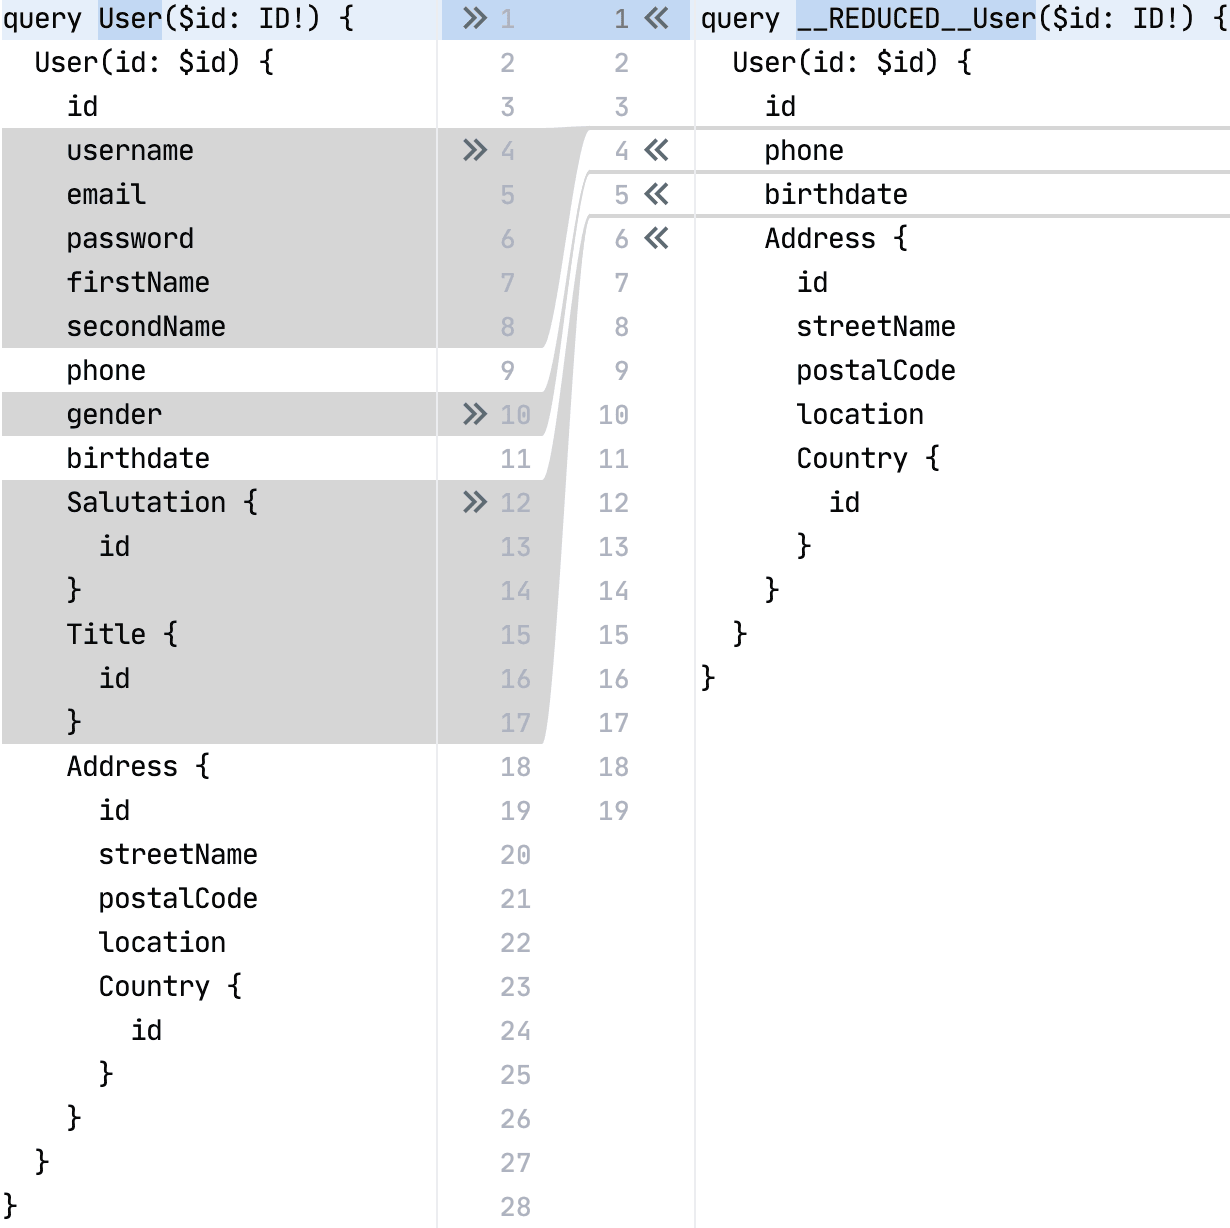
\includegraphics[width=0.65\linewidth]{images/reduction-graphql-examples/compare-user-reduced-user.png}
  \caption{A comparison of the original user- and reduced user-query.}\label{fig:applied-methods:comparison-user-reduced-user}
  \end{figure}
\fi



